\documentclass{article}
\usepackage[utf8]{inputenc}
\usepackage{graphicx,wrapfig}
\usepackage{amsmath}
\usepackage{titling}
\usepackage{pdflscape}
\usepackage[export]{adjustbox}
\usepackage{float}
\usepackage{booktabs} % To thicken table lines
\usepackage{adjustbox}
\usepackage{caption}
\usepackage[colorlinks=false,hidelinks]{hyperref}

\setlength{\droptitle}{-10em}
\pagestyle{empty}

\title{Lab. 4 - Clustering di dati medici}
\author{Ballarin Simone, Gobbo Alessio, Rossi Daniel}
\date{June 2019}

\begin{document}

\maketitle

\section*{Domanda 1}
\begin{center}
	\begin{figure}[H]
		\hspace*{1.5cm}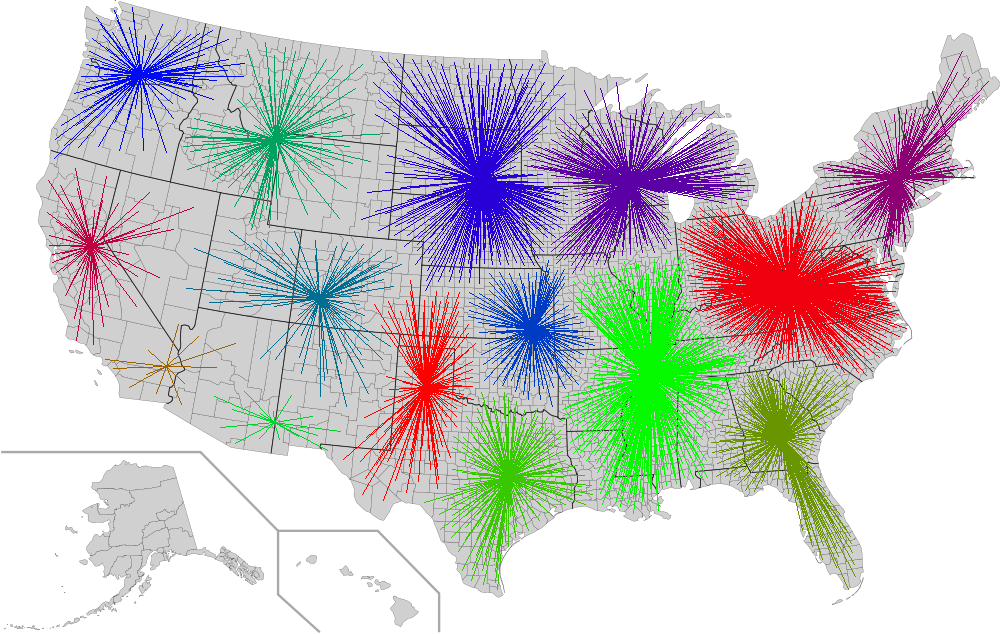
\includegraphics[width=0.8\linewidth, valign=t]{figures/Domanda1}
		\caption*{15 cluster ottenuti con clustering gerarchico su 3108 contee.}
	\end{figure}
\end{center}

\section*{Domanda 2}
\begin{center}
	\begin{figure}[H]
		\hspace*{1.5cm}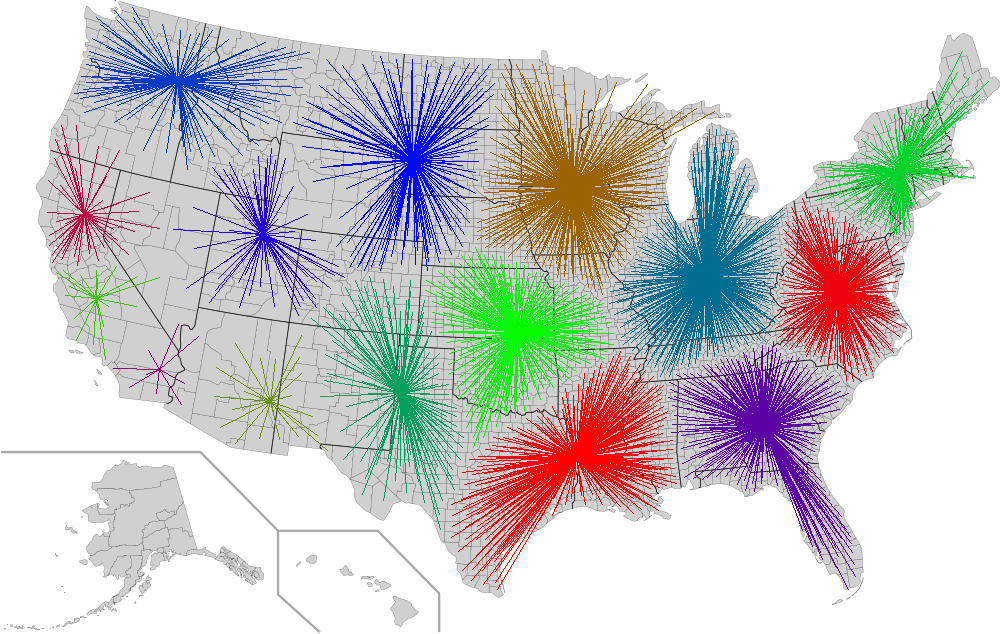
\includegraphics[width=0.8\linewidth, valign=t]{figures/Domanda2}
		\caption*{15 cluster ottenuti con clustering Kmeans su 3108 contee con 5 iterazioni.}
										
	\end{figure}
\end{center}

\section*{Domanda 3}
Dati $q$ il numero di iterazioni di \textit{Kmeans}, $k$ il numero di cluster e $n$ la cardinalità dell'insieme dei punti, possiamo quantificare le seguenti complessità dei due algoritmi di clustering:
\begin{itemize}
	\item La complessità del clustering gerarchico è $O(n\,h(n))$, dove $h(n)$ è la complessità della ricerca dei punti più vicini.
	      Questa ricerca è stata effettuata con la funzione \textit{FastestClosestPair}, la quale ha complessità $O(n\,log(n))$;
	      Quindi complessivamente il clustering gerarchico ha complessità $O(n^2\,log(n))$.
	\item La complessità di \textit{Kmeans} invece è di $O(q\,n\,k)$. 
\end{itemize}

\noindent Ipotizzando quindi $q$ e $k$ fattori molto piccoli, quindi trascurabili come segue $q \approx 1$ e $k \approx 1$, giungiamo alla conclusione che 
la complessità del clustering gerarchico rimanga inalterata, mentre \textit{Kmeans} giunga a $O(n)$.\\
Da quanto appena esposto risulta evidente come \textit{Kmeans} sia, in termini asintotici, e considerando $q$ e $k$ insignificanti, significativamente più efficiente.

\section*{Domanda 4}
\begin{center}
	\begin{figure}[H]
		\hspace*{1.5cm}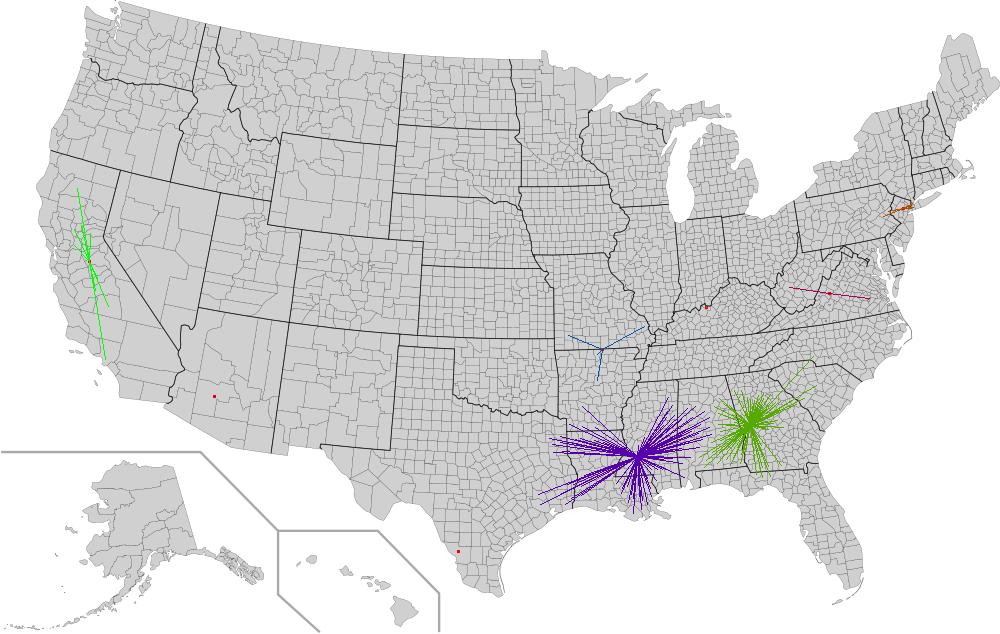
\includegraphics[width=0.8\linewidth, valign=t]{figures/Domanda4}
		\caption*{9 cluster ottenuti con clustering gerarchico su 212 contee.}
										
	\end{figure}
\end{center}
\section*{Domanda 5}
\begin{center}
	\begin{figure}[H]
		\hspace*{1.5cm}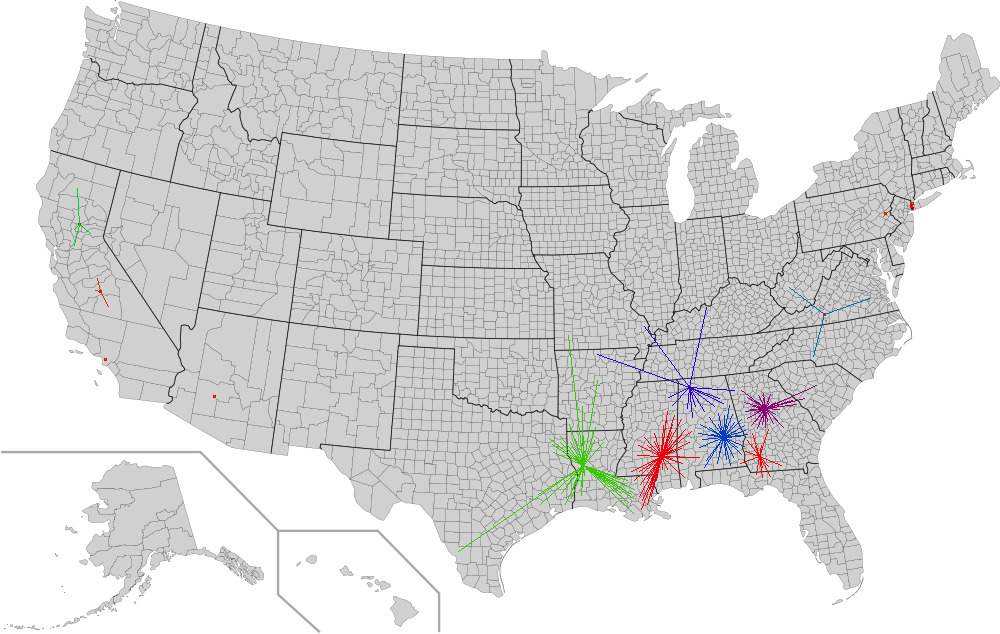
\includegraphics[width=0.8\linewidth, valign=t]{figures/Domanda5}
		\caption*{9 cluster ottenuti con clustering Kmeans su 212 contee con 5 iterazioni.}
	\end{figure}
\end{center}
\section*{Domanda 6}
L'algoritmo di clustering gerarchico con 9 cluster in output e 212 contee presenta un valore di dispersione pari a $1.9675E+11$.\\
Invece, Kmeans applicato al set di dati con 212 contee, con 5 iterazioni e 9 cluster è affetto da una distorsione pari a $9.5383E+10$.

\section*{Domanda 7}

\begin{wrapfigure}[12]{l}{3cm}
	\vspace*{-0.5cm}
	\centering
	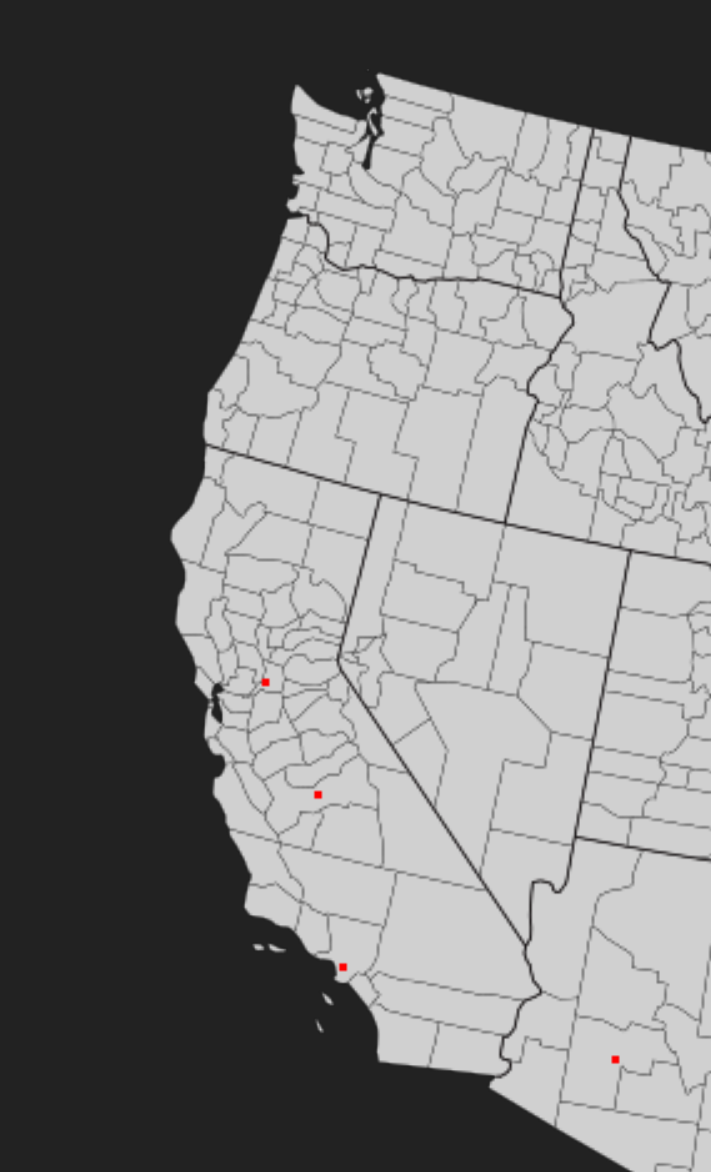
\includegraphics[width=1.0\linewidth]{figures/costa_bis}
	\caption*{Città più popolose della costa occidentale.}
\end{wrapfigure}
Relativamente alla costa occidentale, il clustering Gerarchico si presenta con un cluster contenente tutti i punti presi in esame. Kmeans, invece, raggruppa in maniera più uniforme attuando un'alterazione minima rispetto ai centroidi di partenza.\\
Considerando la geografia della costa occidentale, notiamo essere presenti 4 tra le 9 contee più popolose dell'intero paese.
Questo porta Kmeans a partire e anche a finire con 4 centroidi in quella zona.
Il clustering gerarchico, invece, partendo con ogni contea come centroide non introduce nessuna precedenza alla costa occidentale (che in Kmeans è data dalla presenza di città molto popolose).\\

\noindent Come evidenziato dalla \hyperlink{fig:test}{\textbf{tabella}}, il clustering Gerarchico migliora sensibilmente la propria distorsione all'aumentare del numero di cluster finale.
Ciò ci permette di affermare che l'elevata agglomerazione in un solo centroide è da inputare ad una scarsa cardinalità dei cluster di output.


\section*{Domanda 8}
Kmeans richiede conoscenza a priori sulla topologia dei punti (in quanto i centroidi iniziali devono essere selezionati) e sul numero di cluster che si vuole ottenere.\\
Queste due informazioni, specialmente la prima, introducono un bias molto forte sul risultato finale.
Quindi riteniamo che l'algoritmo di clustering gerarchico sia quello che necessiti di meno supervisione umana, ma più controllo sulla bonta della soluzione finale.\\
Al fine di capire l'importanza di controllare la bontà della soluzione finale generata da Kmeans, si vuole far notare come da prove empiriche emerga che con un piccolo numero di punti il clustering gerarchico attui pochi accorpamenti, proponendo risultati ad alta dispersione. In questi contesti risulta più efficace Kmeans. Se infatti a quest'ultimo vengono forniti il numero di cluster finali ed un numero di iterazioni, anche non troppo alto, si può ottenere un risultato con dispersione inferiore. \\ 
Il clustering gerarchico, invece, può essere interrotto non appena la distorsione superi una data soglia.

\section*{Domanda 9}
Di seguito vengono riportati tre grafici, ognuno facente riferimento ad un dataset di dimensioni differenti (in sequenza 212, 562 e 1041 contee). \\
Ogni grafico esprime sull'asse delle ordinate il valore della metrica dispersione al variare del numero di cluster in output.\\
\subsection*{212 contee, clustering gerarchico e Kmeans}
\hypertarget{fig:test}{}
\begin{figure}[H]
	\hspace*{-1cm}\begin{minipage}{0.55\linewidth}
	\centering	
	\begin{tabular}{lrr}
	\toprule
	{} & hierarchical & kmeans       \\
	k  &              &              \\
	\midrule
	6  & 3.551330e+11 & 1.942049e+11 \\
	7  & 2.119842e+11 & 1.216588e+11 \\
	8  & 2.079946e+11 & 1.208180e+11 \\
	9  & 1.967522e+11 & 9.538277e+10 \\
	10 & 1.458858e+11 & 7.612516e+10 \\
	11 & 7.333959e+10 & 6.940441e+10 \\
	12 & 7.298695e+10 & 5.684592e+10 \\
	13 & 6.292566e+10 & 5.105708e+10 \\
	14 & 3.749038e+10 & 4.506050e+10 \\
	15 & 3.075468e+10 & 4.144032e+10 \\
	16 & 3.052271e+10 & 3.658922e+10 \\
	17 & 1.965371e+10 & 3.645427e+10 \\
	18 & 1.899275e+10 & 1.849405e+10 \\
	19 & 1.890876e+10 & 1.754538e+10 \\
	20 & 1.449351e+10 & 1.612765e+10 \\
	\bottomrule
\end{tabular}

	\end{minipage}
	\begin{minipage}{0.7\linewidth}
		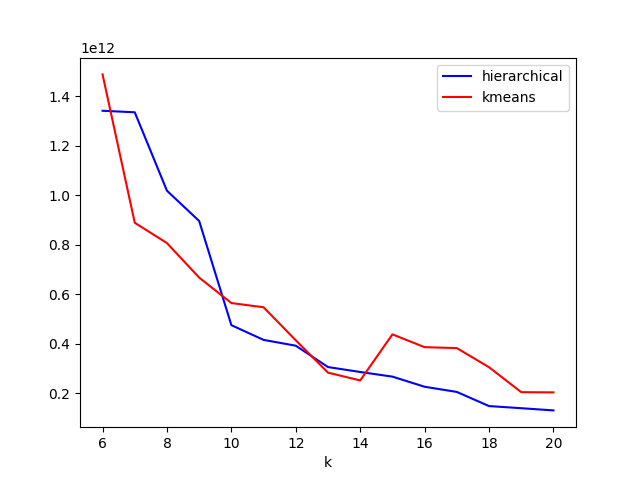
\includegraphics[width=1.0\linewidth, valign=t]{figures/output562}
		\caption*{Grafico dispersione del dataset con 212 contee.}
	\end{minipage}
\end{figure}
\subsection*{562 contee, clustering gerarchico e Kmeans}

\begin{figure}[H]
	\hspace*{-1cm}\begin{minipage}{0.55\linewidth}
	\centering
	\begin{tabular}{lrr}
\toprule
{} &  hierarchical &        kmeans \\
k  &               &               \\
\midrule
6  &  1.341235e+12 &  1.488108e+12 \\
7  &  1.335053e+12 &  8.888297e+11 \\
8  &  1.018233e+12 &  8.067753e+11 \\
9  &  8.959328e+11 &  6.674107e+11 \\
10 &  4.751940e+11 &  5.644963e+11 \\
11 &  4.157366e+11 &  5.475082e+11 \\
12 &  3.922197e+11 &  4.140267e+11 \\
13 &  3.060045e+11 &  2.835009e+11 \\
14 &  2.860567e+11 &  2.519570e+11 \\
15 &  2.673648e+11 &  4.380518e+11 \\
16 &  2.264599e+11 &  3.862867e+11 \\
17 &  2.055237e+11 &  3.826377e+11 \\
18 &  1.484142e+11 &  3.053247e+11 \\
19 &  1.397912e+11 &  2.046021e+11 \\
20 &  1.309398e+11 &  2.037350e+11 \\
\bottomrule
\end{tabular}
 
	\end{minipage}
	\begin{minipage}{0.7\linewidth}
		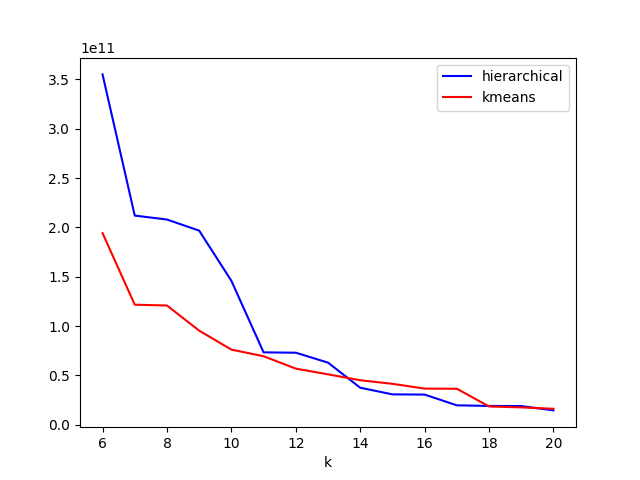
\includegraphics[width=1.0\linewidth, valign=t]{figures/output212}
		\caption*{Grafico dispersione del dataset con 562 contee.}
	\end{minipage}
\end{figure}
\subsection*{1041 contee, clustering gerarchico e Kmeans }
\begin{figure}[H]
	\hspace*{-1cm}\begin{minipage}{0.55\linewidth}
	\centering
	\begin{tabular}{lcc}
	\toprule
	k  & Gerarchico   & Kmeans       \\
	\midrule
	6  & 2.497247e+12 & 2.524928e+12 \\
	7  & 2.222620e+12 & 1.568259e+12 \\
	8  & 1.375668e+12 & 1.180744e+12 \\
	9  & 1.140418e+12 & 1.089885e+12 \\
	10 & 8.687074e+11 & 8.469028e+11 \\
	11 & 8.461629e+11 & 7.754888e+11 \\
	12 & 8.407428e+11 & 7.742760e+11 \\
	13 & 8.309796e+11 & 7.727588e+11 \\
	14 & 6.195937e+11 & 7.119578e+11 \\
	15 & 5.753650e+11 & 6.438951e+11 \\
	16 & 5.010563e+11 & 6.243352e+11 \\
	17 & 4.670626e+11 & 4.585690e+11 \\
	18 & 4.216256e+11 & 4.254108e+11 \\
	19 & 3.703708e+11 & 4.204501e+11 \\
	20 & 3.666637e+11 & 3.834206e+11 \\
	\bottomrule
\end{tabular}

	\end{minipage}
	\begin{minipage}{0.7\linewidth}
		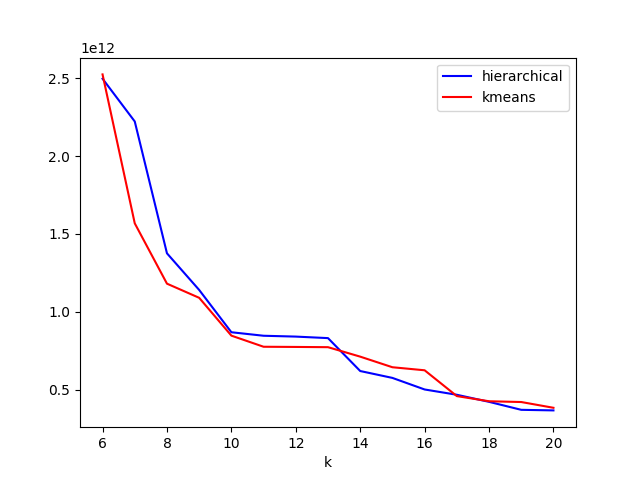
\includegraphics[width=1.0\linewidth, valign=t]{figures/output1041}
		\caption*{Grafico dispersione del dataset con 1041 contee.}
										
	\end{minipage}
\end{figure}

\section*{Domanda 10}
Come si può osservare dai grafici riportati nella domanda nove, in tutti i dataset nessuno dei due algoritmi riesce ad ottenere risultati migliori dell'altro al variare del valore di $k$.\\
Nell'istanza da 212 contee notiamo come con bassi valori di $k$ entrambi gli algoritmi hanno alti valori di dispersione, con Kmeans che si comporta generalmente meglio, tra $k=[10,14]$ abbiamo un comportamento altalenante, ed infine da $k=15$ in poi il gerarchico diventa stabilmente il migliore.\\
Nell'istanza da 562 contee vediamo come fino a $k=14$ cluster Kmeans ottiene una dispersione migliore, da qui in poi il clustering gerarchico ottiene risultati migliori per poi convergere con Kmeans nell'intervallo $k=[18,20]$.\\
Nell'istanza da 1041 contee notiamo che i due algoritmi in termini di dispersione sono analoghi.
\end{document}

